% vim: set textwidth=78 autoindent:

\subsection{Dxf2Shp Converter Plugin}
\subsection{Extension de conversion Dxf2Shp}

% when the revision of a section has been finalized, 
% comment out the following line:
%\updatedisclaimer

% The dxf2shape converter plugin allows to convert vector data from DXF to Shapefile 
% format. It is very simple to handle and provides following functionality as 
% shown in Figure \ref{fig:dxf2shape_dialog}.
L'extension de conversion Dxf2Shp permet de convertir des donn\'ees vectorielles du format DXF au format shapefile (SHP).
Tr\`es facile \`a utiliser, elle pr\'esente les fonctionnalit\'es pr\'esent\'ees dans la Figure \ref{fig:dxf2shape_dialog}).

% \begin{itemize}
% \item \textbf{Input DXF file}: Enter path to the DXF file to be converted
% \item \textbf{Output Shp file}: Enter desired name of the shape file to be created
% \item \textbf{Output file type}: specifies the type of the output Shapefile. Currently supported is polyline, polygone and point.
% \item \textbf{Export text labels}: If you enable this checkbox, an additional Shapefile points layer will be created, and the associated dbf table will contain information about the "TEXT" fields found in the dxf file, and the text strings themselves.
% \end{itemize}
\begin{itemize}
\item \textbf{Fichier DXF} : Entrez l'adresse du fichier DXF \`a convertir.
\item \textbf{Fichier SHP de sortie}: Entrez le nom souhait\'e du fichier shape \`a cr\'eer.
\item \textbf{Type de fichier de sortie}: Sp\'ecifiez le type du fichier shape. Les formats impl\'ement\'es pour le moment sont polyligne, polygone et point.
\item \textbf{Exporter les \'etiquettes} : Si vous cochez cette case, une couche suppl\'ementaire sera cr\'e\'ee (points), et la table dbf associ\'ee contiendra des informations \`a propos des champs "TEXT" trouv\'es dans le fichier DXF, et les cha\^ines de caract\`eres elles-m\^emes.
\end{itemize}

% \begin{figure}[ht]
   % \begin{center}
   % \caption{Dxf2Shape Converter Plugin \nixcaption}\label{fig:dxf2shape_dialog}\smallskip
   % 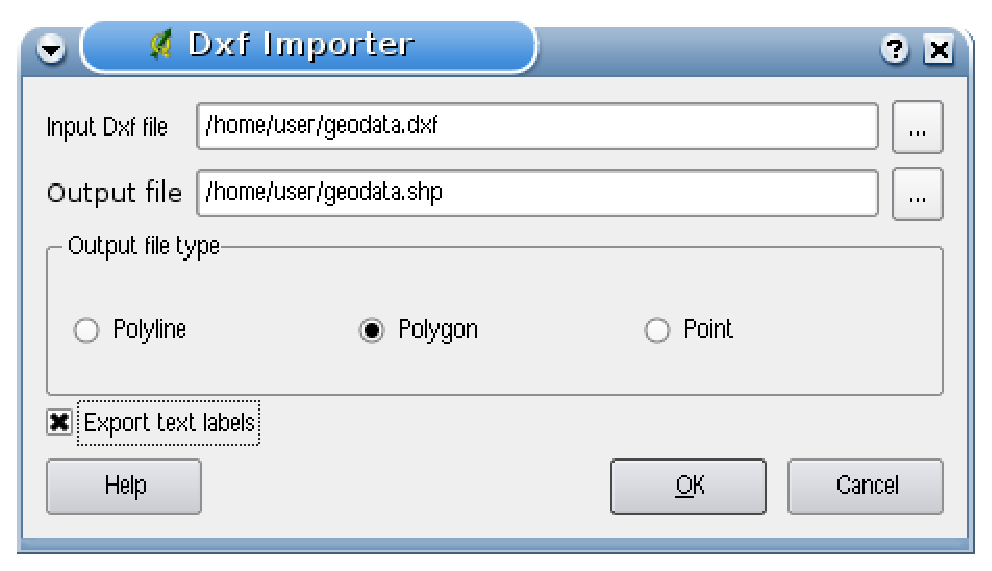
\includegraphics[clip=true, width=13cm]{dxf2shape_dialog}
% \end{center}  
% \end{figure}
\begin{figure}[ht]
   \begin{center}
   \caption{Le convertisseur Dxf2Shp\nixcaption}\label{fig:dxf2shape_dialog}\smallskip
   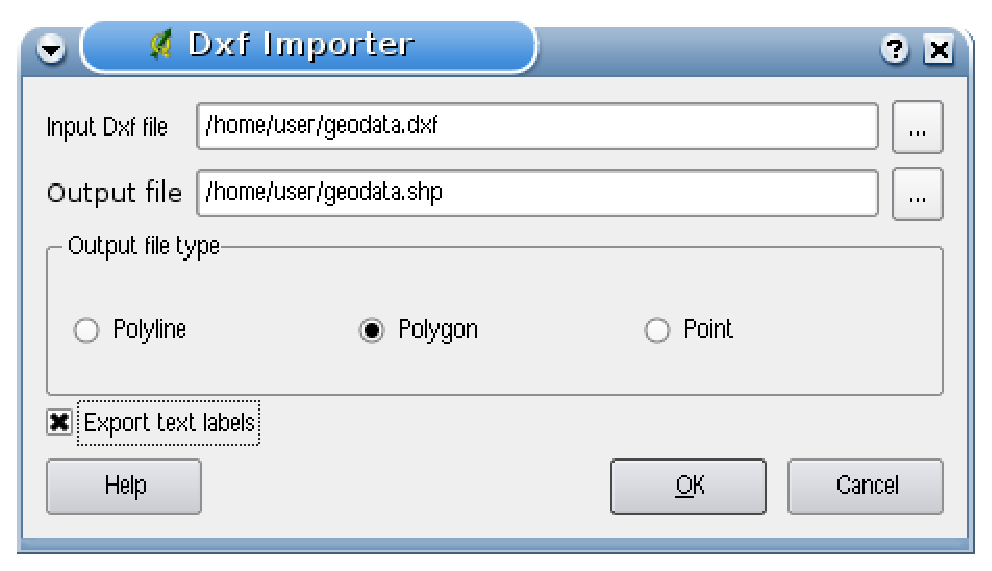
\includegraphics[clip=true, width=13cm]{dxf2shape_dialog}
\end{center}  
\end{figure}

% \begin{enumerate}
  % \item Start QGIS, load the Dxf2Shape plugin in the Plugin Manager (see Section 
  % \ref{sec:load_core_plugin}) and click on the \toolbtntwo{dxf2shp_converter}{Dxf2Shape Converter} 
  % icon which appears in the QGIS toolbar menu. The Dxf2Shape plugin dialog appears as shown in Figure \ref{fig:dxf2shape_dialog}.
  % \item Enter input DXF file, a name for the output Shapefile and the Shapefile type.
  % \item Enable the \checkbox{Export text labels} checkbox, if you want to create an extra point layer with labels.
  % \item Click \button{Ok}. 
% \end{enumerate}
\begin{enumerate}
  \item D\'emarrez QGIS, chargez l'extension Dxf2Shp dans le gestionnaire d'extensions (voir la Section 
  \ref{sec:load_core_plugin}) et cliquez sur l'ic\^one \toolbtntwo{dxf2shp_converter}{Convertisseur Dxf2Shp} 
  qui apparait dans les barres d'outils de QGIS. La bo\^ite de dialogue de l'extension Dxf2Shp appara\^it, comme indiqu\'e dans la Figure 
  \ref{fig:dxf2shape_dialog}.
  \item Entrez le fichier d'origine DXF, choisissez un nom pour le fichier SHP de sortie et le type de fichier shape.
  \item Cochez la case \checkbox{Exporter les \'etiquettes}, si vous souhaitez cr\'eer une couche suppl\'ementaire comprenant les \'etiquettes.
  \item Cliquez sur \button{Ok}. 
\end{enumerate}

\newpage